\chapter{Entonación de las metaheurísticas}
\label{apendiceA}
\lhead{Apéndice A. \emph{Entonación de las metaheurísticas}}.

\section{Entonación de GGA}

Los parámetros de los que depende GGA son: el número de iteraciones, el tamaño de la población y la probabilidad de cruce. En la tabla \ref{table-ap-gga} se presentan los diferentes valores evaluados para cada metaheurística. En este sentido, se realizó un estudio factorial para determinar el impacto de cada valor por separado y la interacción entre valores de diferentes parámetros.

\begin{table}[h!]
\centering
\begin{tabular}{l c}
\hline
\textsc{Parámetro} & \textsc{Valores Evaluados} \\
\hline
\hline
Iteraciones & 100\ \ \textbf{1000}\ \ 10000 \\
Población   & 10\ \ 20\ \ 30\ \ 40\ \ \textbf{50} \\
Prob. de Cruce & 0.5\ \ 0.6\ \ 0.75\ \ \textbf{0.9}\ \ 1.0\\
\hline
\end{tabular}
\caption{Valores evaluados para los parámetros de GGA}
\label{table-ap-gga}
\end{table}

En la figura \ref{fig-ap-gga} se presentan los resultados obtenidos de este estudio. Resulta evidente la existencia de un impacto inversamente proporcional entre el tamaño de población y el error de validación. Con una población de tamaño 50, GGA logra los mejores resultados.
Adicionalmente, los mejores resultados se obtienen mediante el uso de una probabilidad de cruce igual a 1.0 o 0.9, favoreciendo ligeramente a la selección de una probabilidad igual a 0.9.
Sin embargo, los resultados en función del número de iteraciones no son concluyentes, puesto que los resultados exhiben un comportamiento errático. Se selecciona un número de iteraciones igual a 1000.

\begin{figure}[h!]
\centering
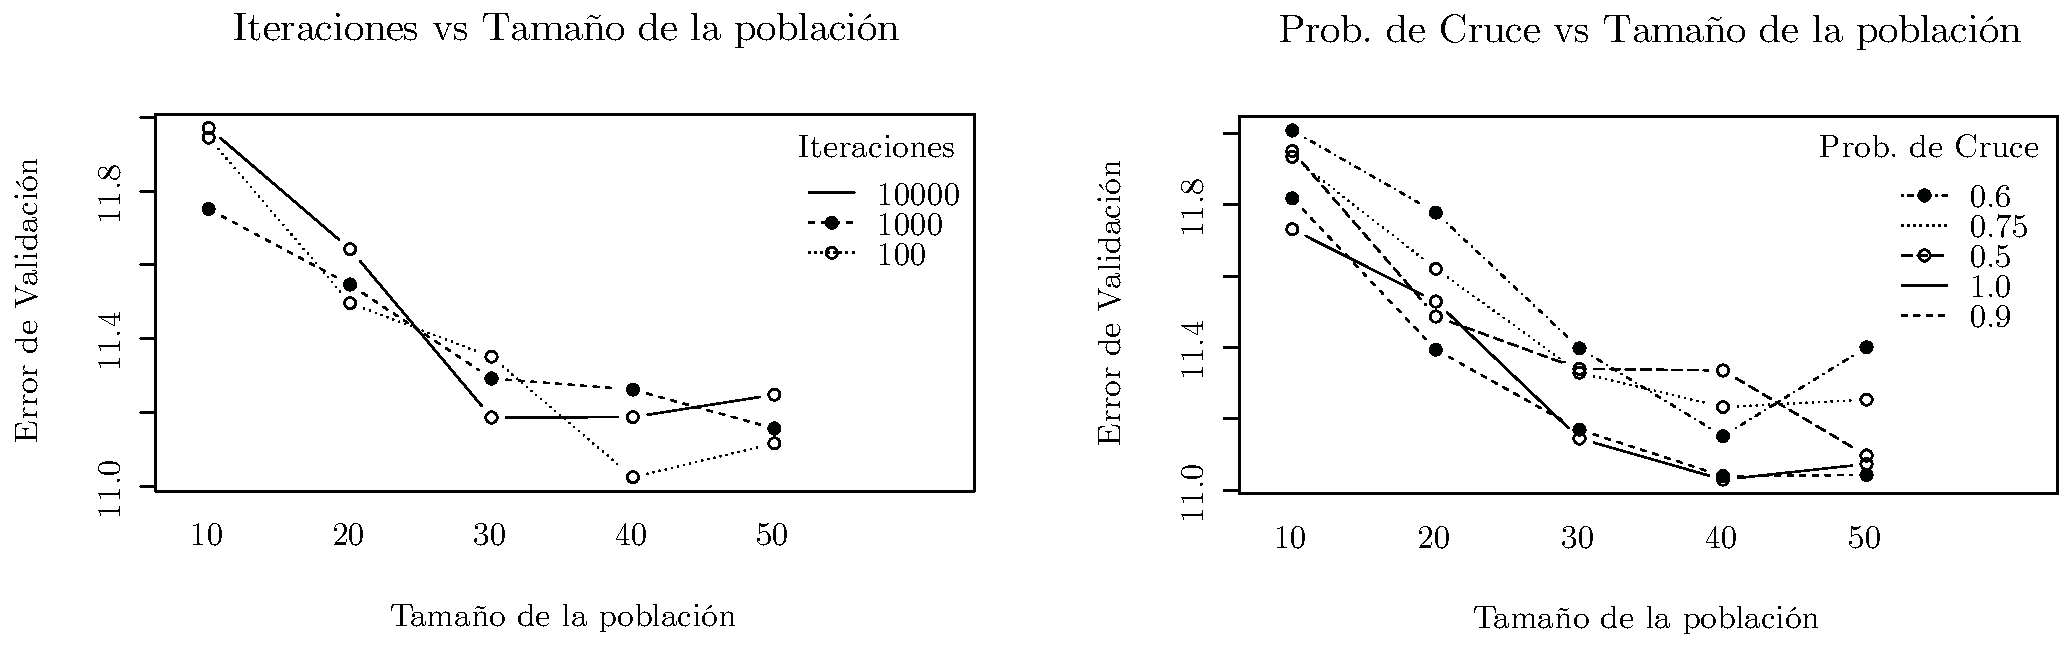
\includegraphics[width=\textwidth]{apendice-gga.pdf}
\caption{Resultados de entonación de GGA}
\label{fig-ap-gga}
\end{figure}

\section{Entonación de SGA}

SGA depende de los mismos parámetros que GGA. Por esta razón, se evalúan los mismos valores, descritos en la tabla \ref{table-ap-sga}. A partir de estos niveles de evaluación, se realiza un estudio factorial entre todos los parámetros.

\begin{table}[h!]
\centering
\begin{tabular}{l c}
\hline
\textsc{Parámetro} & \textsc{Valores Evaluados} \\
\hline
\hline
Iteraciones & 100\ \ \textbf{1000}\ \ 10000 \\
Población   & 10\ \ 20\ \ \textbf{30}\ \ 40\ \ 50 \\
Prob. de Cruce & 0.5\ \ 0.6\ \ 0.75\ \ 0.9\ \ \textbf{1.0}\\
\hline
\end{tabular}
\caption{Valores evaluados para los parámetros de SGA}
\label{table-ap-sga}
\end{table}

Al comparar los resultados presentados en la figura \ref{fig-ap-sga}, resulta evidente el efecto positivo de aumentar el número de iteraciones en SGA. Sin embargo, a pesar de que los resultados favorecen ampliamente el uso de 10000 iteraciones, esto implica un aumento de un orden de magnitud en el tiempo de ejecución de la metaheurística. Esto lleva a la selección de un número de iteraciones intermedio (1000) que genere soluciones aceptables sin incurrir en altos costos de cómputo.

Adicionalmente, los resultados presentados en función del tamaño de la población usada, llevan a concluir que este parámetro no influye significativamente en el proceso de búsqueda de SGA. Se selecciona el nivel medio, igual a 30 individuos.

Por último, el efecto la probabilidad de cruce es poco claro. Se decide seleccionar una probabilidad de cruce igual a 1.0 para asegurar la generación de nuevos individuos en cada iteración.

\begin{figure}[h!]
\centering
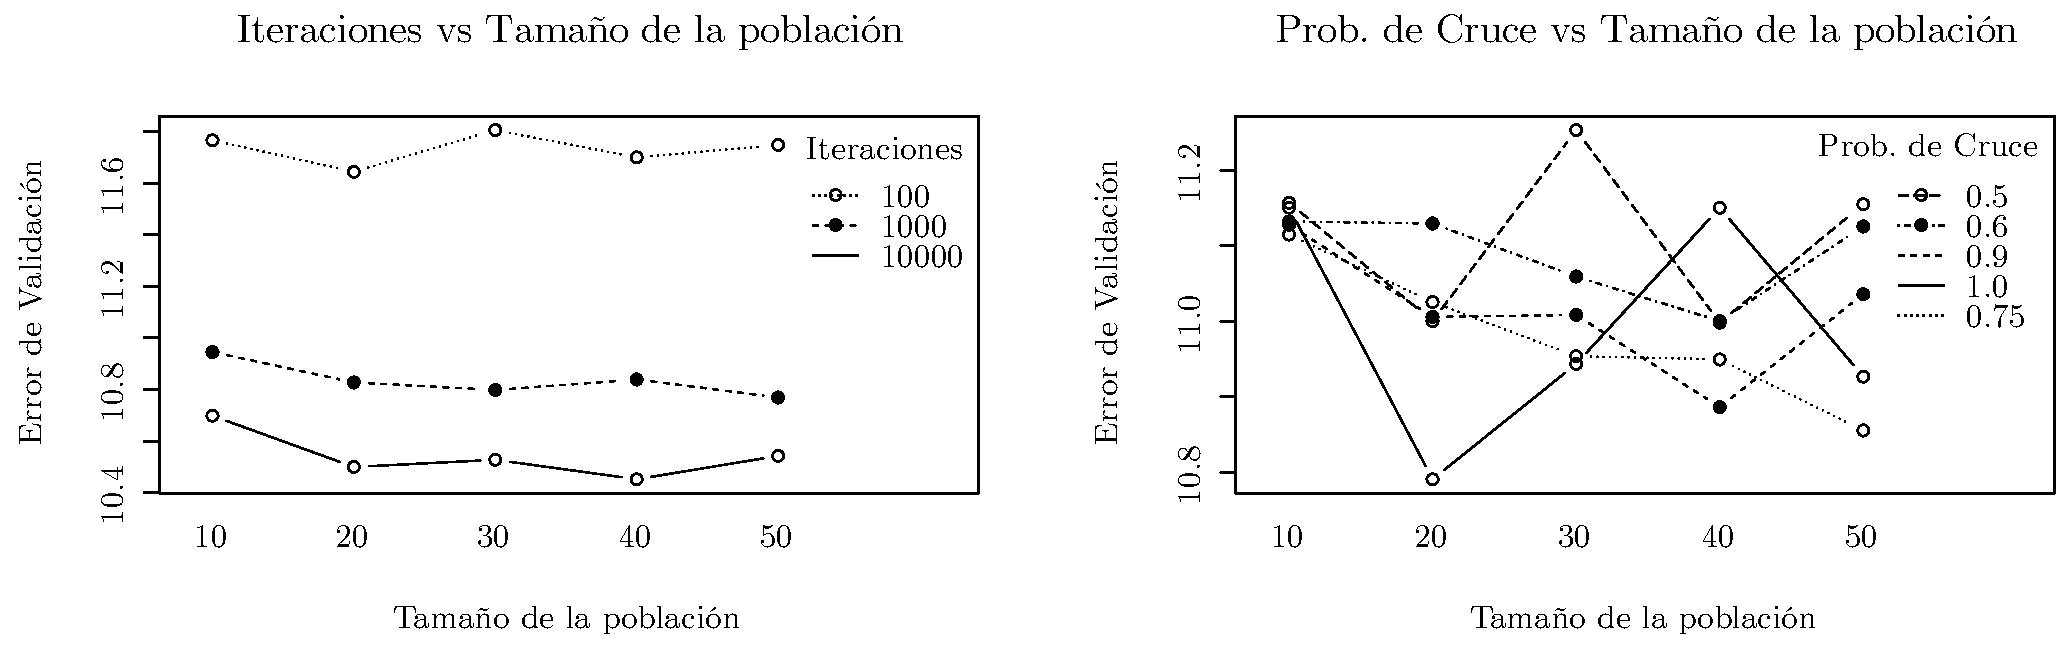
\includegraphics[width=\textwidth]{apendice-sga.pdf}
\caption{Resultados de entonación de SGA}
\label{fig-ap-sga}
\end{figure}

\section{Entonación de CHC}

CHC es la metaheurística con menos parámetros que entonar. Tan solo depende del número de iteraciones y el tamaño de la población. Los valores evaluados son descritos en la tabla \ref{table-ap-chc}.

\begin{table}[h!]
\centering
\begin{tabular}{l c}
\hline
\textsc{Parámetro} & \textsc{Valores Evaluados} \\
\hline
\hline
Iteraciones & 100\ \ \textbf{1000}\ \ 10000 \\
Población   & 10\ \ 20\ \ \textbf{30}\ \ 40\ \ 50 \\
\hline
\end{tabular}
\caption{Valores evaluados para los parámetros de CHC}
\label{table-ap-chc}
\end{table}

Los resultados presentados en la figura \ref{fig-ap-chc} son claros y las conclusiones evidentes. El comportamiento de la metaheurística luego de 1000 o 10000 iteraciones es muy similar, y es poco dependiente del tamaño de la población. Se escoge un tamaño de población medio (igual a 30) y un número de iteraciones igual 1000 para reducir el tiempo de ejecución.

\begin{figure}[h!]
\centering
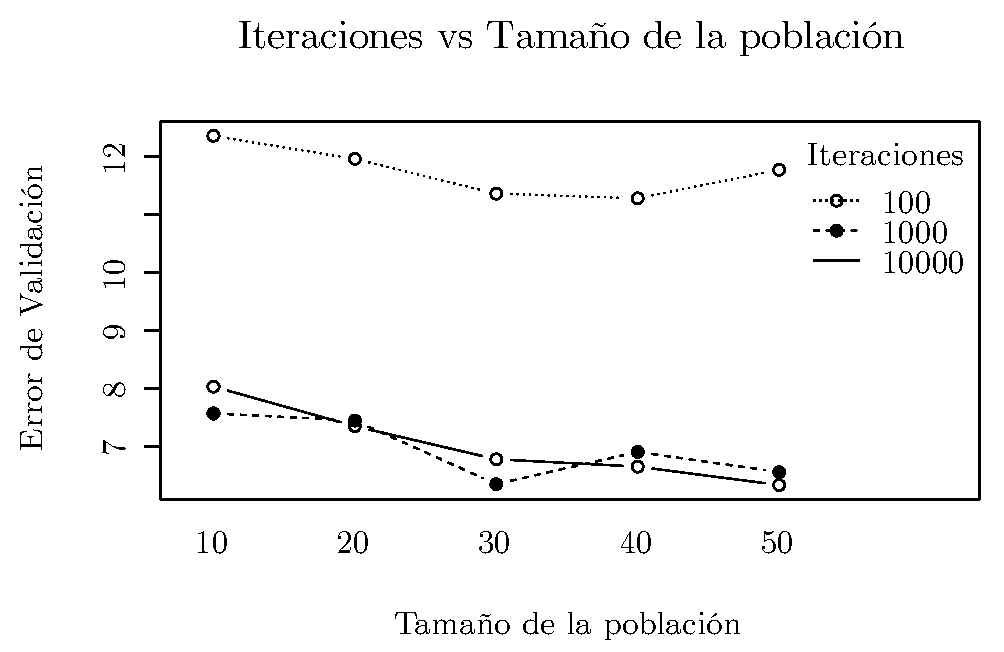
\includegraphics[width=0.5\textwidth]{apendice-chc.pdf}
\caption{Resultados de entonación de CHC}
\label{fig-ap-chc}
\end{figure}

\section{Entonación de PBIL}

La entonación de PBIL resulta más complicada, debido a que depende de un mayor número de parámetros. En la tabla \ref{table-ap-pbil} se describen los valores evaluados para cada parámetro. Se excluye de este estudio el valor de \emph{Mutation Shift}, que se mantiene en un valor bajo. Con los niveles descritos, se realiza un estudio factorial.

\begin{table}[h!]
\centering
\begin{tabular}{l c}
\hline
\textsc{Parámetro} & \textsc{Valores Evaluados} \\
\hline
\hline
Iteraciones & 100\ \ \textbf{1000}\ \ 10000 \\
Población   & 10\ \ 20\ \ 30\ \ \textbf{40}\ \ 50 \\
Learning Rate & \textbf{0.1}\ \ 0.05\ \ 0.01 \\
Negative Learning Rate & 0.075\ \ 0.05\ \ \textbf{0.01} \\
\hline
\end{tabular}
\caption{Valores evaluados para los parámetros de PBIL}
\label{table-ap-pbil}
\end{table}

De los resultados obtenidos y presentados en la figura \ref{fig-ap-pbil}, se derivan las siguientes conclusiones:
\begin{itemize}
\item El tamaño de la población y el número de iteraciones influyen significativamente en la disminución del error de validación. Aplicando 1000 iteraciones, los mejores resultados son obtenidos con poblaciones de tamaño 40.
\item Existe una relación importante entre los valores de \emph{Learning Rate} y el \emph{Negative Learning Rate}. Los mejores resultados se obtienen de la combinación de 0.1 para \emph{Learning Rate} y 0.01 para \emph{Negative Learning Rate}.
\end{itemize}

\begin{figure}[h!]
\centering
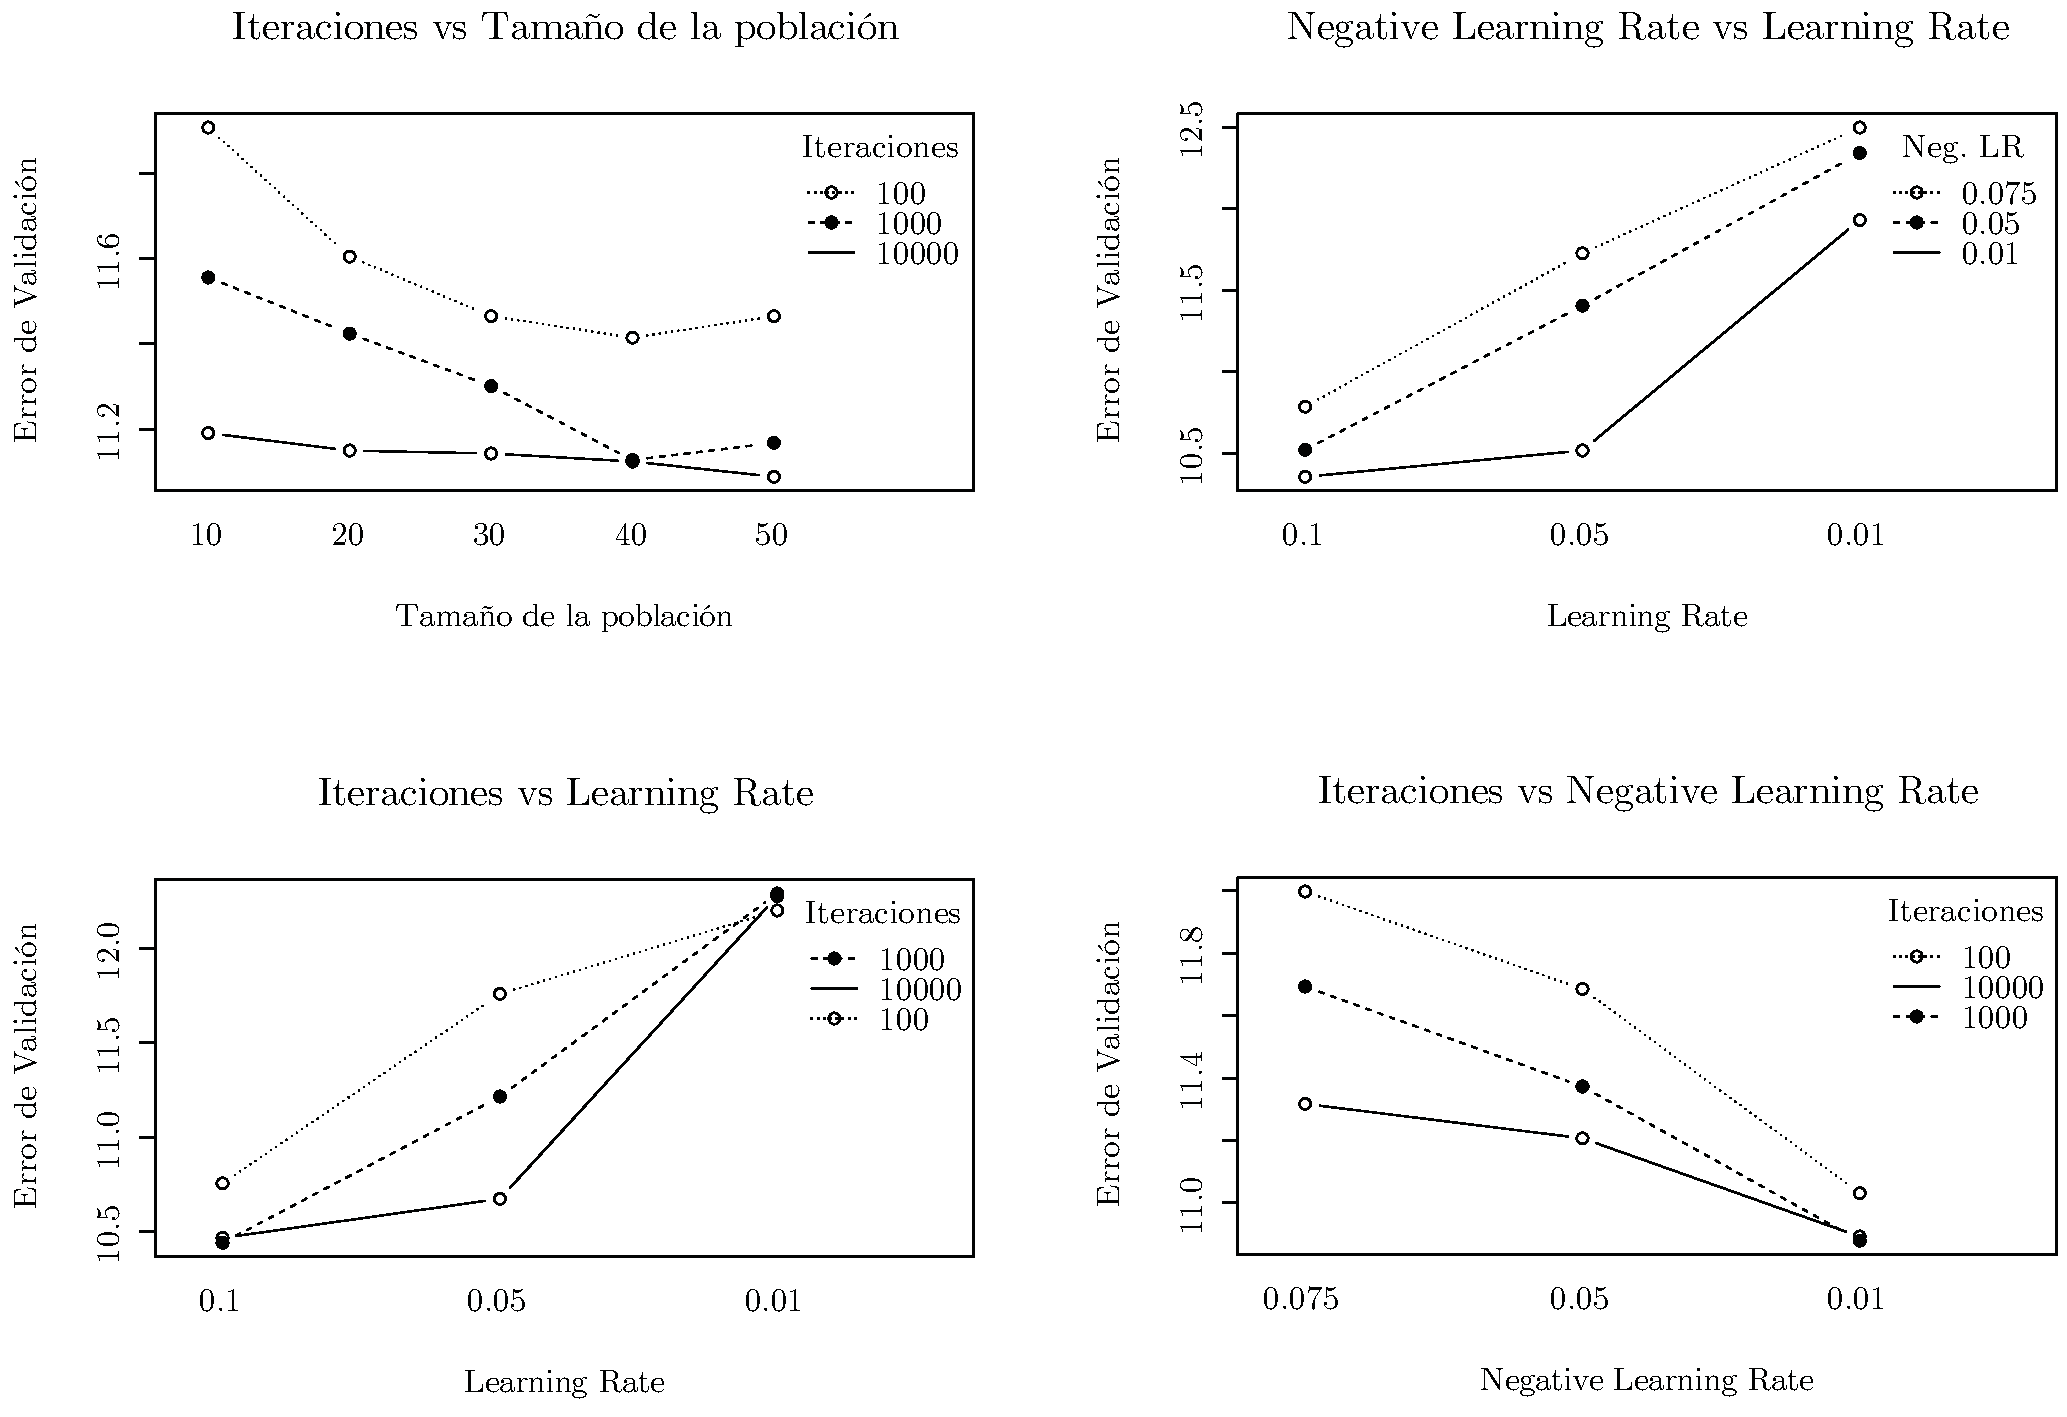
\includegraphics[width=\textwidth]{apendice-pbil.pdf}
\caption{Resultados de entonación de PBIL}
\label{fig-ap-pbil}
\end{figure}

\section{Entonación de PSO}

En la tabla \ref{table-ap-pso} se describen los valores utilizados para evaluar el impacto de algunos de los parámetros de los que depende PSO. El resto de los parámetros fueron fijados con la finalidad de limitar el impacto en tiempo sobre el algoritmo. PSO se vio especialmente afectado en tiempo de ejecución por el número de iteraciones, por lo que se decidió fijar este parámetro en 1000 al igual que el resto de las metaheurísticas. Adicionalmente, debido a que el número de soluciones generadas por PSO en cada iteración es igual al número de partículas por el tamaño de la población, se fijó este último parámetro para evitar un aumento considerable en el tiempo de ejecución. Las constantes $c1$ y $c2$ son toman un valor igual a $\frac{\texttt{vmax}}{2}$ pues no tiene sentido usar valores más altos dado que el vector de velocidad está acotado por $\texttt{vmax}$ (velocidad máxima).

\begin{table}[h!]
\centering
\begin{tabular}{l c}
\hline
\textsc{Parámetro} & \textsc{Valores Evaluados} \\
\hline
\hline
Partículas  & \textbf{5}\ \ 10\ \ 15 \\
Inercia     & \textbf{0.9}\ \ 0.6\ \ 0.3 \\
Velocidad Máxima & 0.5\ \ \textbf{0.2}\ \ 0.05 \\
\hline
\end{tabular}
\caption{Valores evaluados para los parámetros de PSO}
\label{table-ap-pso}
\end{table}

Para los valores de Inercia y Velocidad Máxima, se realizó un estudio factorial, y los resultados son presentados en la figura \ref{fig-ap-pso}. Resulta clara la interacción entre diferentes valores de estos parámetros, donde la combinación de una inercia igual a 0.9 y una velocidad máxima de 0.2 logran los mejores resultados.

El número de partículas fue evaluado de forma independiente. Los resultados obtenidos muestran que no existen diferencias en el uso de diferentes números de partículas. Este parámetro se fija en 5 partículas con la finalidad de disminuir el tiempo de ejecución del algoritmo.

\begin{figure}[h!]
\centering
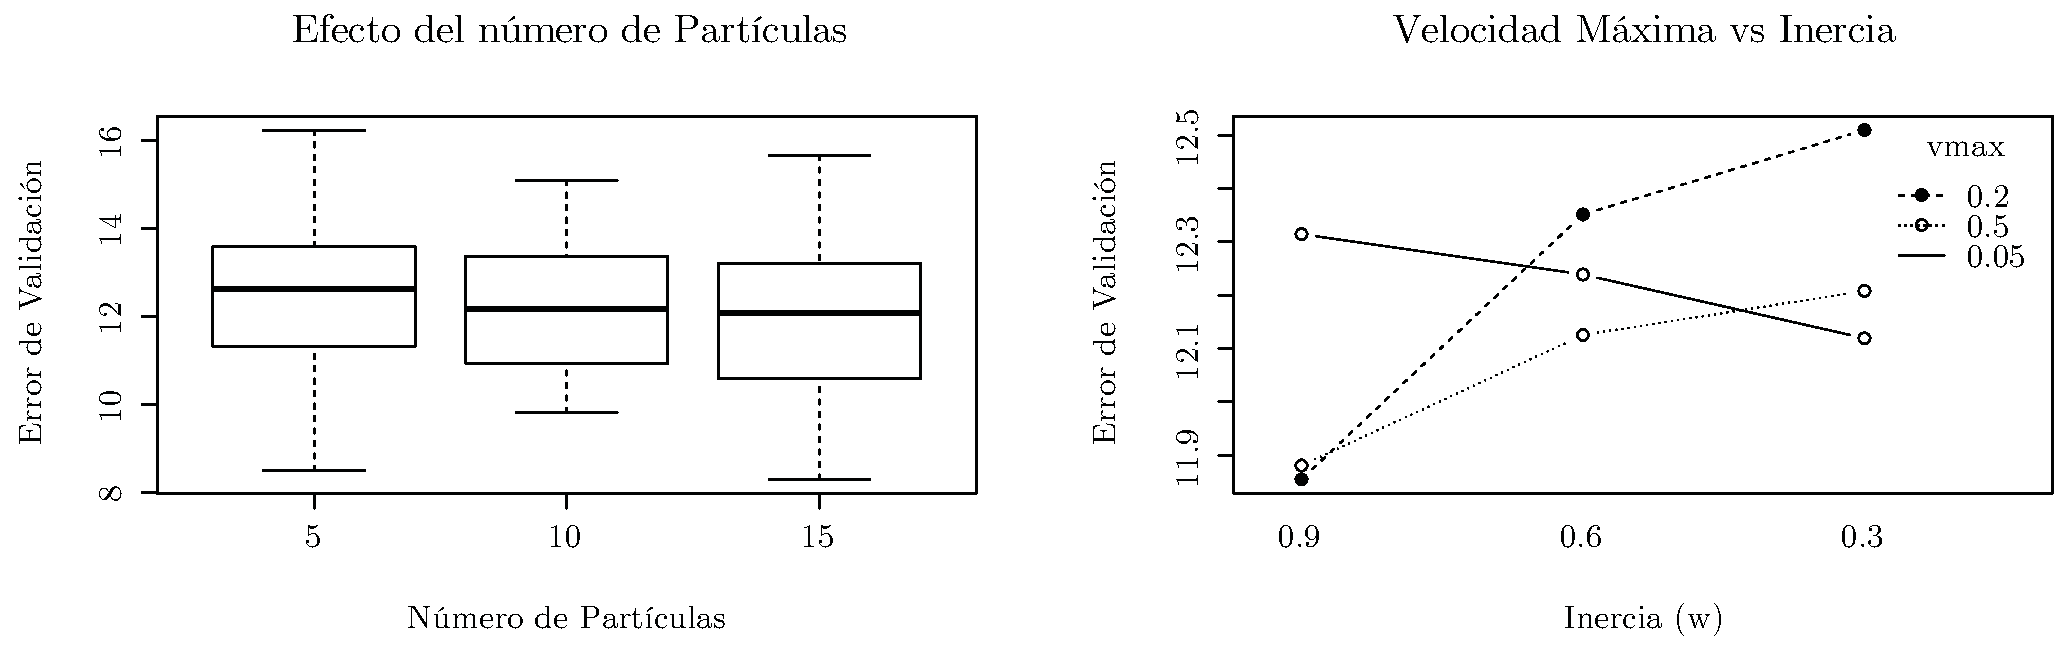
\includegraphics[width=\textwidth]{apendice-pso.pdf}
\caption{Resultados de entonación de PSO}
\label{fig-ap-pso}
\end{figure}
